\documentclass{scrartcl}
\usepackage[a4paper,landscape,left=0.25cm,right=0.25cm,top=0.5cm,bottom=0.5cm]{geometry}
 
\usepackage[]{ifdraft}
\usepackage[]{attachfile}
\usepackage[]{eso-pic}
 
\usepackage[english]{babel}
\usepackage[T1]{fontenc}
\usepackage[utf8]{inputenc}
 
\renewcommand{\familydefault}{\sfdefault}
\RequirePackage[scaled=0.9]{helvet}
\usepackage{tikz}
\usepackage[right]{showlabels}
\usetikzlibrary{positioning}
\pagestyle{empty}
 
\usepackage{xcolor}
 
\usepackage{hyperref}
\usepackage{url}
 
\definecolor{weekendday}{RGB}{240,240,240}
\newcommand{\file}[1]{\textattachfile{#1}{\textcolor{blue}{\LaTeX\ Sourcecode}}}
 
\begin{document}  
 
\AddToShipoutPictureFG*{
  \put(35,10){\footnotesize Uwe Ziegenhagen, ziegenhagen@gmail.com %, \file{\jobname.tex}	
}
}
 
\begin{center}
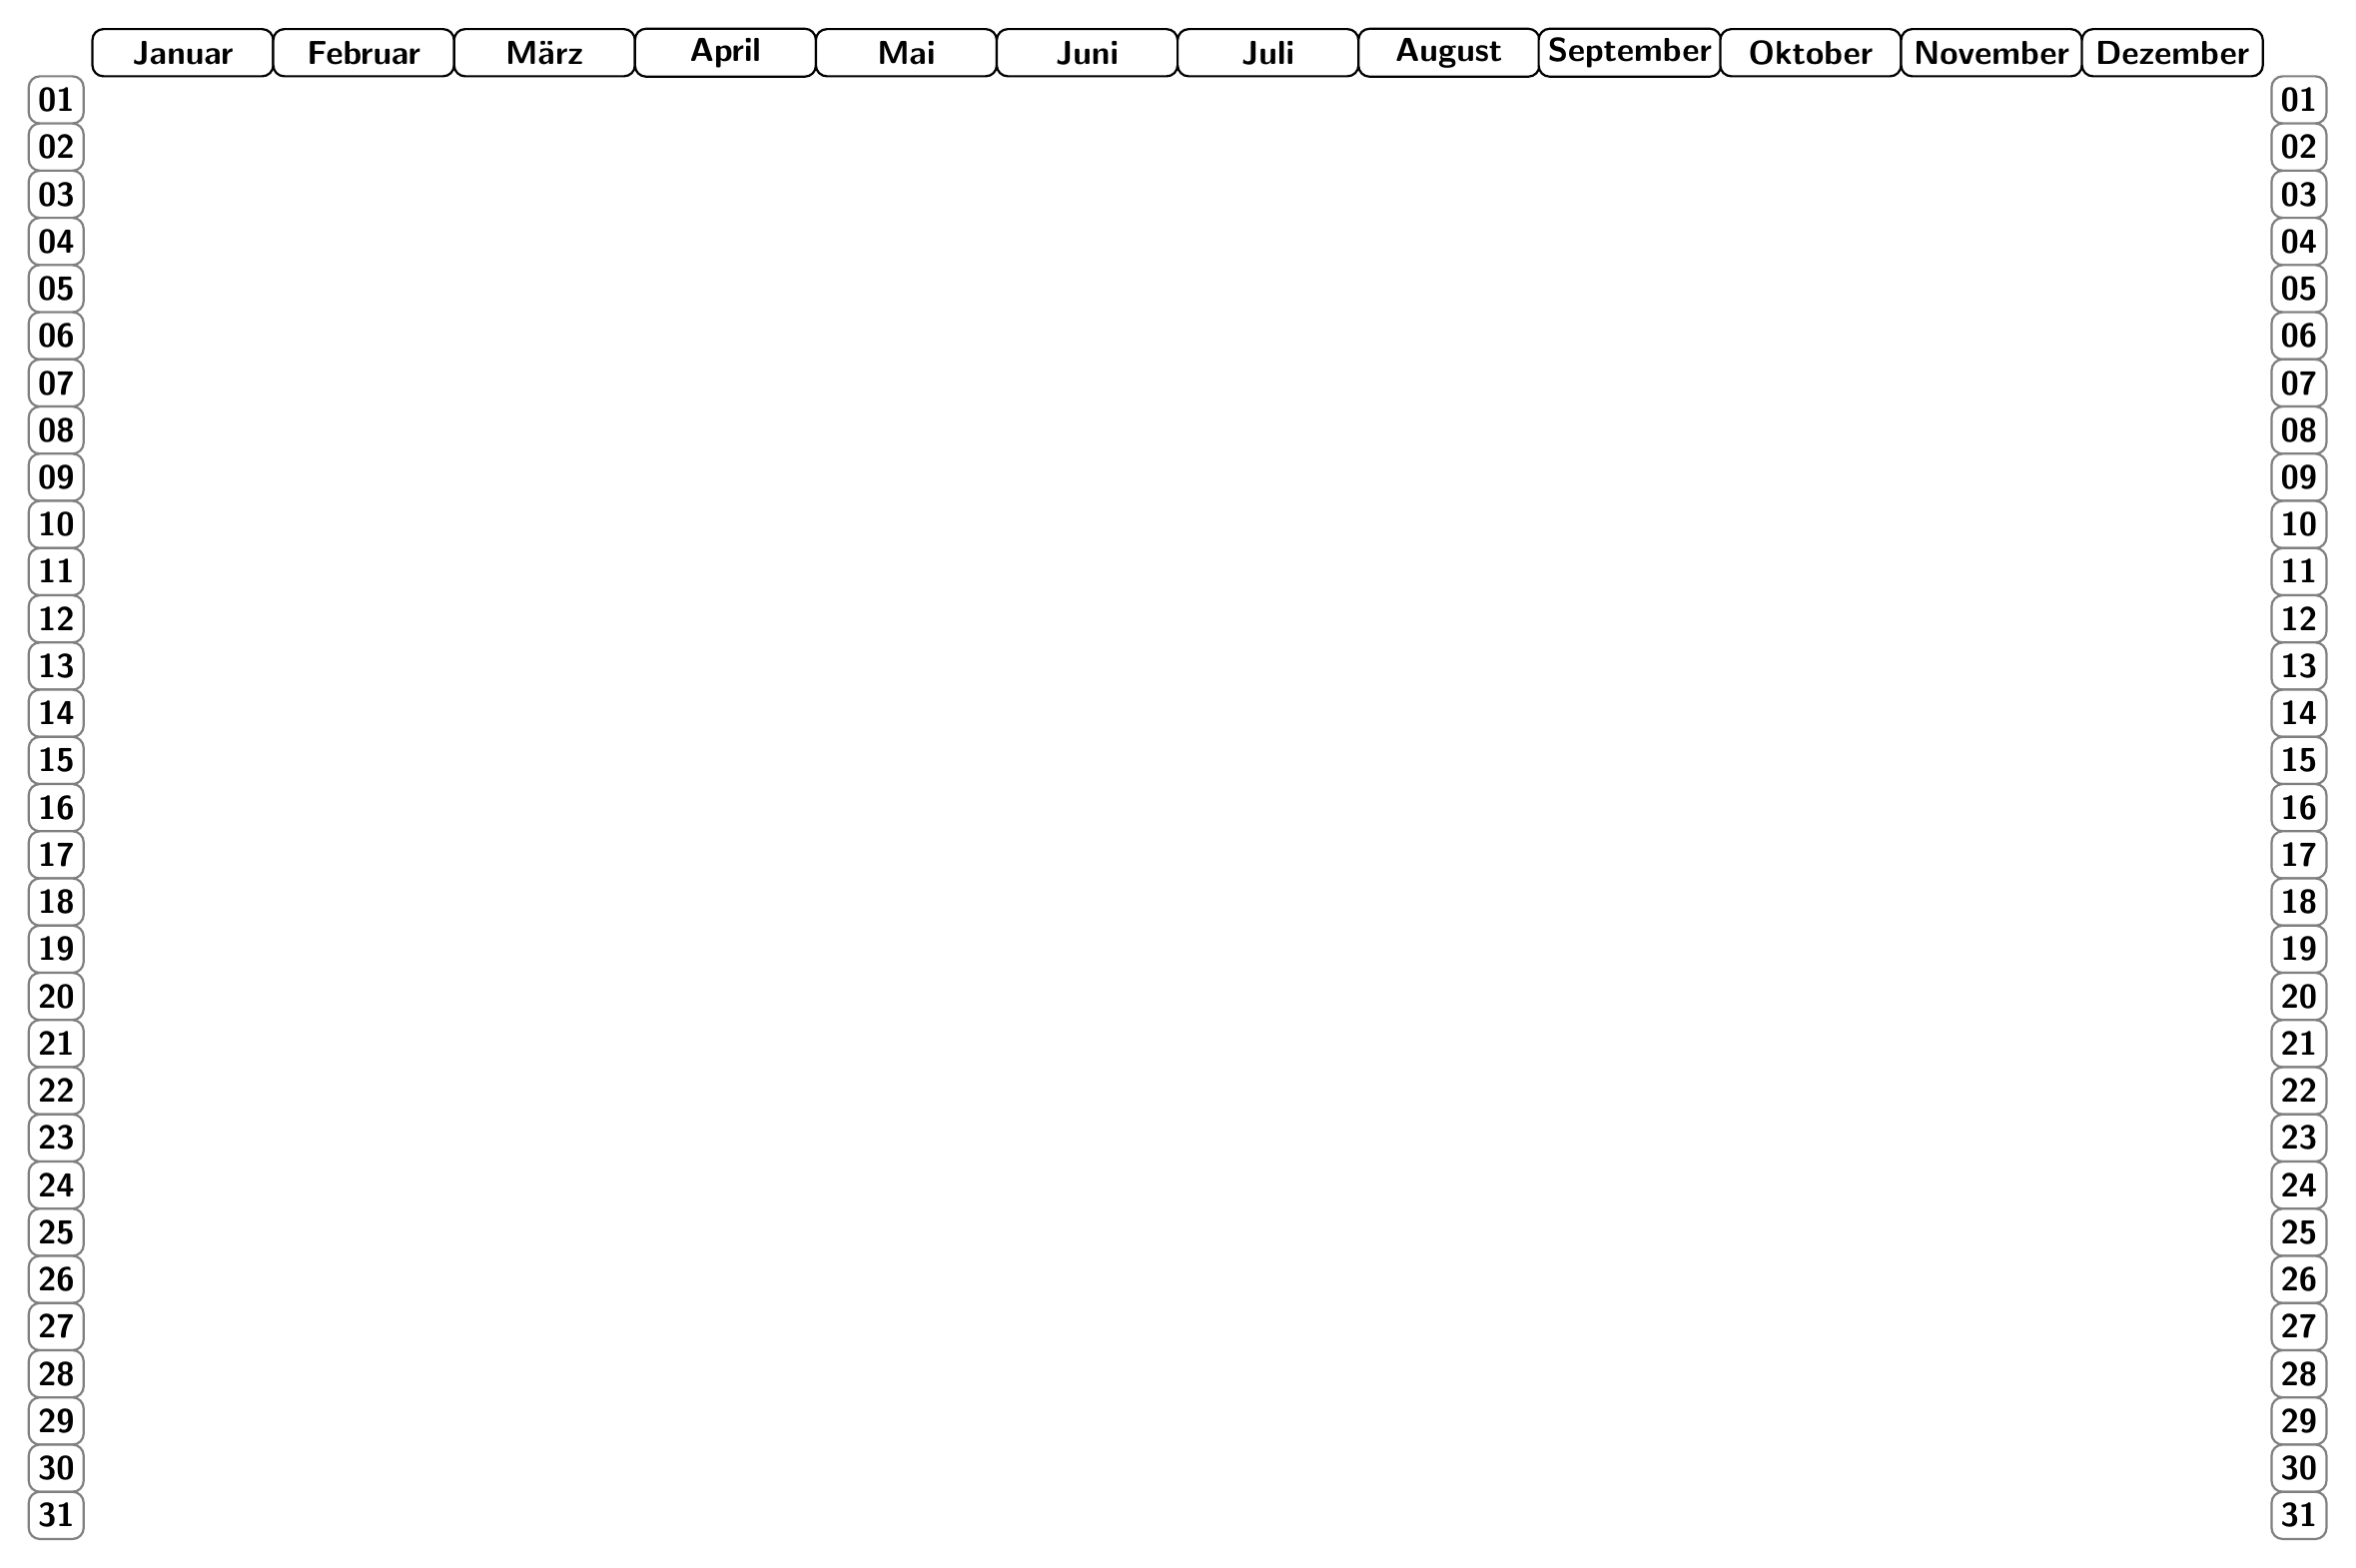
\begin{tikzpicture}
[
    x=23mm,y=6mm,
    mybox/.style={rectangle,rounded corners,minimum width=23mm, minimum height=6mm,align=left},
	month/.style={mybox,align=center,draw=black,align=left,fill=white,thick,font=\bfseries\large},
    date/.style={mybox,draw=gray,fill=white,align=left,thick,minimum width=5mm,font=\bfseries\large},
    workday/.style={mybox,draw=black,text width=1.5cm,font=\bfseries\tiny},
    weekend/.style={mybox,draw=black,text width=1.5cm,fill=weekendday,font=\bfseries\tiny}
]
\node at (0,0) [month] {Januar};
\node at (1,0) [month] {Februar};
\node at (2,0) [month] {März};
\node at (3,0) [month] {April};
\node at (4,0) [month] {Mai};
\node at (5,0) [month] {Juni};
\node at (6,0) [month] {Juli};
\node at (7,0) [month] {August};
\node at (8,0) [month] {September};
\node at (9,0) [month] {Oktober};
\node at (10,0) [month] {November};
\node at (11,0) [month] {Dezember};
 
\node at (-0.7,-1) [date] {01};
\node at (-0.7,-2) [date] {02};
\node at (-0.7,-3) [date] {03};
\node at (-0.7,-4) [date] {04};
\node at (-0.7,-5) [date] {05};
\node at (-0.7,-6) [date] {06};
\node at (-0.7,-7) [date] {07};
\node at (-0.7,-8) [date] {08};
\node at (-0.7,-9) [date] {09};
\node at (-0.7,-10) [date] {10};
\node at (-0.7,-11) [date] {11};
\node at (-0.7,-12) [date] {12};
\node at (-0.7,-13) [date] {13};
\node at (-0.7,-14) [date] {14};
\node at (-0.7,-15) [date] {15};
\node at (-0.7,-16) [date] {16};
\node at (-0.7,-17) [date] {17};
\node at (-0.7,-18) [date] {18};
\node at (-0.7,-19) [date] {19};
\node at (-0.7,-20) [date] {20};
\node at (-0.7,-21) [date] {21};
\node at (-0.7,-22) [date] {22};
\node at (-0.7,-23) [date] {23};
\node at (-0.7,-24) [date] {24};
\node at (-0.7,-25) [date] {25};
\node at (-0.7,-26) [date] {26};
\node at (-0.7,-27) [date] {27};
\node at (-0.7,-28) [date] {28};
\node at (-0.7,-29) [date] {29};
\node at (-0.7,-30) [date] {30};
\node at (-0.7,-31) [date] {31};
 
\node at (11.7,-1) [date] {01};
\node at (11.7,-2) [date] {02};
\node at (11.7,-3) [date] {03};
\node at (11.7,-4) [date] {04};
\node at (11.7,-5) [date] {05};
\node at (11.7,-6) [date] {06};
\node at (11.7,-7) [date] {07};
\node at (11.7,-8) [date] {08};
\node at (11.7,-9) [date] {09};
\node at (11.7,-10) [date] {10};
\node at (11.7,-11) [date] {11};
\node at (11.7,-12) [date] {12};
\node at (11.7,-13) [date] {13};
\node at (11.7,-14) [date] {14};
\node at (11.7,-15) [date] {15};
\node at (11.7,-16) [date] {16};
\node at (11.7,-17) [date] {17};
\node at (11.7,-18) [date] {18};
\node at (11.7,-19) [date] {19};
\node at (11.7,-20) [date] {20};
\node at (11.7,-21) [date] {21};
\node at (11.7,-22) [date] {22};
\node at (11.7,-23) [date] {23};
\node at (11.7,-24) [date] {24};
\node at (11.7,-25) [date] {25};
\node at (11.7,-26) [date] {26};
\node at (11.7,-27) [date] {27};
\node at (11.7,-28) [date] {28};
\node at (11.7,-29) [date] {29};
\node at (11.7,-30) [date] {30};
\node at (11.7,-31) [date] {31};
 
 
% hier kommen die Sachen aus Excel rein
 
\end{tikzpicture}
\end{center}
\end{document}